\documentclass{article}
\usepackage[utf8]{inputenc}
\usepackage[margin=0.5in]{geometry}
\usepackage{graphicx}
\usepackage{amsmath}
\usepackage{ dsfont }

\graphicspath{ {../figs/} }


\title{Problem Set 4: Quantitative Economics (ECON 8185-001)}
\author{Teerat Wongrattanapiboon}
\date{\today}

\begin{document}
	\maketitle
	
	\noindent\textbf{\Large Aiyagari Model with Finite Element Method} \\
	
	Our problem is 
	
	$$\max \mathds{E}\sum_{t=0}^{\infty}\beta^{t}\left[ c_{t}^{1-\mu} - 1 \right] / (1-\mu)$$
	
	$$\text{s.t. } c_{t} + a_{t+1} = wl_{t} + (1+r)a_{t}$$
	
	$$c_{t} \geq 0, a_{t} \geq 0,$$
	
	where $l_{t}$ is assumed to be i.i.d. and well approximated by a Markov chain. In this note, we assume 
	
	\[
  		l_{t+1} = 
  		\begin{cases}
    		l_{low} = 0.2, \pi = 1/2 \\
    		l_{high} = 0.9, \pi = 1/2 
  		\end{cases}
	\]
	
	$$\Pi_{ij} = \begin{bmatrix} 1/2 & 1/2 \\ 1/2 & 1/2 \end{bmatrix},$$
	
	\begin{center}
		\begin{tabular}{| c | c |  }
		\hline
 		Parameter & Value \\
 		\hline 
 		$\beta$ & 0.96 \\
 		\hline 
 		$\mu$ & 3 \\
 		\hline 
 		$w$ & 1 \\
 		\hline 
 		$1+r$ & 1.02 \\
 		\hline 
 		$\zeta$ & 50000 \\
 		\hline    
		\end{tabular}
	\end{center}
	
	The recursive formulation of our problem is
	
	$$V(a_{t}) = \max_{a_{t+1}}\frac{(wl_{i,t} + (1+r)a_{t} - a_{t+1})^{1-\mu} - 1}{1-\mu} + \beta\mathds{E}[V(a_{t+1})]$$
	
	and the FOC and envelope condition imply 
	
	$$(wl_{t} + (1+r)a_{t}-a_{t+1})^{-\mu} = \beta (1+r) \mathds{E}[(wl_{t+1}+(1+r)a_{t+1}-a_{t+2})^{-\mu}]$$
	
	$$(wl_{t} + (1+r)a_{t}-a_{t+1})^{-\mu} - \frac{\beta(1+r)}{2}\left[ (wl_{t+1}^{L}+(1+r)a_{t+1}-a_{t+2})^{-\mu} + (wl_{t+1}^{H}+(1+r)a_{t+1}-a_{t+2})^{-\mu} + \zeta\min(a_{t+1},0)^{2} \right] = 0$$
	
	First we want to represent the saving policy function with linear basis functions. Specifically, we write
	
	\[
  		g^{a}(a_{t},l_{t};\theta) = \sum_{i=1}^{N}\theta_{i}^{l}\psi_{i}(a) =
  		\begin{cases}
    		\theta_{1}^{L}\psi_{1}(a) + ... + \theta_{N}^{L} \psi_{N}(a), \text{ for low} \\
    		\theta_{1}^{H}\psi_{1}(a) + ... + \theta_{N}^{H} \psi_{N}(a), \text{ for high},
  		\end{cases}
	\]
	
	where $N$ is the number of elements and each $\psi$ represents a small tent defined in adjacent points of asset grids. That is, for $i \in \{ 2,3,...,N-1 \}$, we have
	
	\[
  		\psi_{i}(a) =
  		\begin{cases}
    		\frac{a - a_{i-1}}{a_{i} - a_{i-1}} \text{ if } a_{i-1} \leq a \leq a_{i} \\
    		\frac{a_{i+1} - a}{a_{i+1} - a_{i}} \text{ if } a_{i} \leq a \leq a_{i+1} \\
    		0 \hspace{1.5 cm} \text{ else }.
  		\end{cases}
	\]
	
	For elements at the boundary, we have
	
	\[
  		\psi_{1}(a) =
  		\begin{cases}
    		\frac{a_{2} - a}{a_{2} - a_{1}} \text{ if } a_{1} \leq a \leq a_{2} \\
    		0 \hspace{1.5 cm} \text{ else },
  		\end{cases}
	\]
	
	\[
  		\psi_{N}(a) =
  		\begin{cases}
    		\frac{a - a_{N}}{a_{N} - a_{N-1}} \text{ if } a_{N-1} \leq a \leq a_{N} \\
    		0 \hspace{1.5 cm} \text{ else }.
  		\end{cases}
	\]
	
	Below is the plot these linear bases for the grid $A = [0,1,3,6]$:
	
	\begin{figure}[htbp]
		\centering
		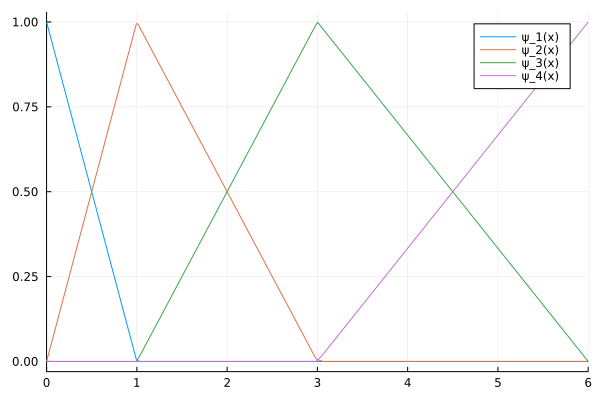
\includegraphics[scale=0.5]{linear_basis.png}
		\caption{Piecewise Linear Basis Functions}
	\end{figure} 
	
	With this saving function, we can also obtain consumption policy function as 
	
	$$g^{c}(a_{t},l_{t};\theta) = Ra_{t} + wl_{t} - g^{a}(a_{t},l_{t};\theta).$$
	
	From the Euler equation above, we can write the residual function as
	
	\begin{align*}
		R(a_{t},l_{t}|\theta) &= (wl_{t} + (1+r)a_{t}-g^{a}(a_{t},l_{t}|\theta))^{-\mu} \\ 
		&- \frac{\beta(1+r)}{2}\Big[ (wl_{t+1}^{L}+(1+r)g^{a}(a_{t},l_{t}|\theta)-g^{a}(g^{a}(a_{t},l_{t}|\theta),l_{t+1}^{L}|\theta))^{-\mu} \\
		&+ (wl_{t+1}^{H}+(1+r)g^{a}(a_{t},l_{t}|\theta)-g^{a}(g^{a}(a_{t},l_{t}|\theta),l_{t+1}^{H}|\theta))^{-\mu} +  \zeta\min(g^{a}(a_{t},l_{t}|\theta),0)^{2} \Big].
	\end{align*}
	
	Then we use the Galerkin choice of weight functions to evaluate the weighted residual of the residual and set it equals to zero. That is,
	
	$$\int\phi_{i}(a)R(a,l|\theta)da = \int\psi_{i}(a)R(a,l|\theta)da = 0, \hspace{0.5cm} \text{ where } i = 1,...,n, l = \{ \text{low}, \text{high}\}$$

	\noindent\textbf{\Large Algorithm and Results} \\
	
	To summarize, the main algorithm is as follows: \\
	
	\hspace{0.5cm} 1) Make a ``proper" guess of $\theta^{j} = \{ \theta_{1}^{L},...,\theta_{n}^{L},\theta_{1}^{H},...,\theta_{n}^{L} \}$.\\
	
	\hspace{0.5cm} 2) Over the $2$-dimensional grids of $a$ and $l$, evaluate $g^{a}(a,l;\theta)$ and $R(a,l|\theta)$. \\
	
	\hspace{0.5cm} 3) Stack all numerical integrals $\int\psi_{i}(a)R(a,l|\theta)da$ into a system of equations $G(\theta^{j}) = 0$ and apply Newton update until $\theta$ converges. \\
	
	Note that I construct $8$ points on the asset grid between $0$ and $6$, with more points clustered near zero to capture binding borrowing constraint. The plot of the estimated saving policy function for two states of labor is as follows:
	
	\begin{figure}[htbp]
		\centering
		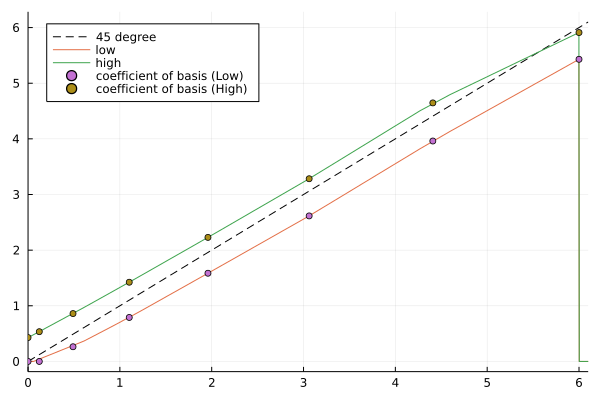
\includegraphics[scale=0.5]{aiyagari.png}
		\caption{Optimal Saving Function with FEM}
	\end{figure} 
	
	
	
\end{document}